\documentclass[../main.tex]{subfiles}

\begin{document}
\subsection{Introduction}
Before we discuss our process of selection for the scheme used to numerically solve the linear shallow-water equations, it is important to understand the idea of a \textit{conservative form} of a hyperbolic partial-differential equation. First we state the conservative form:
\begin{gather}\label{eq:consv}
	\frac{\partial u}{\partial t} + \nabla \cdot \vec F(u) = 0,
\end{gather}
where $u$ is the \textit{density of the conserved quantity}, and $\vec F (u)$ is the \textit{density flux}. Note that the actual form of $\vec F(u)$ is dependent on the original hyperbolic equation that has been converted into this form. Since $u$ is a density, we will denote its corresponding quantity $\mathbf{u}$ defined by:
\begin{gather}\label{eq:dens}
	\mathbf{u} = \int_V u\hspace*{0.10 cm} dV,
\end{gather}
where $V$ denotes the spatial domain. In physics, a \textit{conservation law} requires that some measurable property of a system does not change with respect to time. For example, the conservation of mass (ignoring energy) requires that any system with perfectly balanced mass transfers, or net-zero mass flux along its boundaries, cannot change its total mass over time. To illustrate the connection between such a conservation law and the conservative form of a hyperbolic equation, we present a short derivation proving the conservation of the quantity $\mathbf{u}$. To start, integrate both sides of the conservative form \ref{eq:consv} term-by-term over the spatial domain $V$:
\begin{gather}\label{eq:int}
	\int_V \frac{\partial u}{\partial t} dV + \int_V \nabla \cdot \vec F(u)\hspace*{0.10 cm} dV = 0.
\end{gather}
Now, we apply Leibniz's rule to change the order of differentiation in the first integral:
\begin{gather}\label{eq:s1}
	\int_V \frac{\partial u}{\partial t} dV = \frac{d}{dt} \int_V u\hspace*{0.10 cm} dV.
\end{gather}
Then, we use the divergence theorem on the second integral, which states that integrating the divergence of the vector field, $\nabla \cdot \vec F(u)$, over the spatial domain $V$ is equal to integrating the vector field over the spatial domain's boundary $A$:
\begin{gather}\label{eq:s2}
	\int_V \nabla\cdot F(u)\hspace*{0.10 cm} dV = \int_A \vec F( u) \cdot \vec n \hspace*{0.10 cm}dA,
\end{gather}
where $\vec n$ is the outward-pointing unit vector along the boundary $A$ (see figure~\ref{fig:domain}). By substituting \ref{eq:s1} and \ref{eq:s2} into \ref{eq:int}, one obtains
\begin{gather}\label{eq:cq}
	\frac{d}{dt} \int_V u \hspace*{0.10 cm} dV =- \int_A \vec F(u) \cdot \vec n \hspace*{0.10 cm}dA.
\end{gather}
Thus, the time derivative of $\mathbf{u}$ (see \ref{eq:dens}) in $V$ is equal to the net flux across the boundary $A$ (the second integral). Note that the unit vectors $\vec n$ are outward-pointing along $A$, meaning that $-\vec n$ must be inward-pointing. Thus, this equation does not necessarily say that $\mathbf{m}$ is conserved: it is a more general statement that $\mathbf{m}$ can only change if there is non-zero net flux along the boundary $A$.
\begin{figure}[h]
	\centering
	\fbox{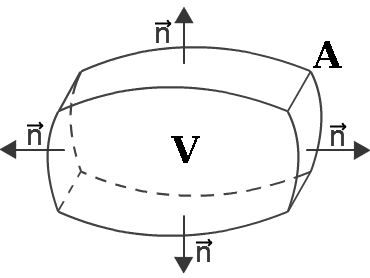
\includegraphics[width=0.50\textwidth]{div}}
	\caption{A spatial domain $\Omega$ and the unit vectors $\vec n$ along its boundary $\partial\Omega$.}
	\label{fig:domain}
\end{figure}

\noindent Now we return to the law of conservation of mass to provide practical intuition regarding \ref{eq:cq}. Assume that the physical system in question is a mass distribution $m$ over some spatial domain $V$, and some mass transfer $\vec F(m)$ within $V$ as well as along $A$. We may state the law of conservation of mass in this case using our previous result \ref{eq:cq}:
\begin{gather}\label{eq:massconsv}
    \frac{d}{dt} \int_V m\hspace*{0.10 cm} dV = - \int_A \vec F(m) \cdot \vec n \hspace*{0.10 cm}dA.
\end{gather}
This offers a clearer picture of the significance of the conserved quantity, as in this case it is the total mass $\mathbf{m}$ of the system:
\begin{gather*}
    \mathbf{m} = \int_V m \hspace*{0.10 cm }dV,
\end{gather*}
In the case where the system is isolated with respect to mass transfers, we know that the flux $A$ is zero everywhere along the boundary:
\begin{gather*}
    \vec F(m) = 0,\quad\text{along } A.
\end{gather*}
This implies that
\begin{gather*}
    \int_A \vec F(m) \cdot \vec n \hspace*{0.10 cm}dA = 0,\quad\text{as } \vec F(m) = 0\text{ along } A.\\
\end{gather*}
Thus, by the statement \ref{eq:massconsv}, we have
\begin{gather*}
    \frac{d}{dt}\int_V m\hspace*{0.10 cm} dV = \frac{d}{dt}\mathbf{m} = 0,
\end{gather*}
that is: the total mass of our system does not change with respect to time. If a system cannot gain or lose mass, the total mass does not change. However, our statement of \ref{eq:massconsv} allows for a more general result: if the net flux along the boundary is zero, we have:
\begin{gather*}
    \int_A \vec F(m) \cdot \vec n \hspace*{0.10 cm}dA = 0.
\end{gather*}
This implies by \ref{eq:massconsv} that the total mass, yet again, cannot change in time. If a system is given some mass but the exactly same amount of mass is removed from the system, the total mass does not change even though the system is not closed with respect to mass transfers along its boundary. Further, if we know the net flux, then we know exactly how the total mass $\mathbf{m}$ will change in time.

\subsection{The Conservative Form of The Shallow-Water Equations}
First we derive the conservative form of the 1D Shallow-Water Equations. The 1D form of the equation:
\begin{gather}\label{eq:1d_sw}
	\frac{\partial^2 u}{\partial t^2} = \frac{\partial }{\partial x}\left( gH\frac{\partial u}{\partial x}\right)
\end{gather}
We convert to flux-conservative form by defining two substitution variables:
\begin{gather*}
	\left.
	\begin{aligned}
		\alpha &= \frac{\partial u}{\partial x}\\
		\gamma &= \frac{\partial u}{\partial t}
	\end{aligned}
	\right\}
	\Rightarrow
	\mathbf{U} = \begin{bmatrix}\alpha \\ \gamma \end{bmatrix}.
\end{gather*}
Our goal is to decouple the equation~\ref{eq:1d_sw} into a system of two equations. This is accomplished by taking derivatives of the above defined substitution variables with respect to time, and applying the law of the equivalence of mixed partials:
\begin{gather*}
	\begin{aligned}
		\frac{\partial \alpha}{\partial t} &= \frac{\partial}{\partial t}\frac{\partial u}{\partial x} = \frac{\partial}{\partial x}\frac{\partial u}{\partial t}=\frac{\partial \gamma}{\partial x},\\
		\frac{\partial \gamma}{\partial t} &=\frac{\partial}{\partial t}\frac{\partial \gamma}{\partial t}=\frac{\partial^2 u}{\partial t^2}=\frac{\partial }{\partial x}\left( gH\alpha\right).
	\end{aligned}
\end{gather*}
This leaves us with the system:
\begin{gather*}
	\frac{\partial }{\partial t}
	\begin{bmatrix}
		\alpha \\ \gamma
	\end{bmatrix}
	+
	\begin{bmatrix}
		\partial_x & 0\\
		0 & \partial_x 
	\end{bmatrix}
	\left(
	\begin{bmatrix}
		0 & 1\\
		-gH & 0
	\end{bmatrix}
	\begin{bmatrix}
		\alpha \\
		\gamma
	\end{bmatrix}
	\right)
	=
	\mathbf{0},
\end{gather*}
which is written succinctly as:
\begin{gather*}
	\frac{\partial \mathbf{U}}{\partial t} + \nabla\cdot\mathbf{F}(\mathbf{U}) = \mathbf{0}.
\end{gather*}
\end{document}
